\documentclass[11pt]{article}
\usepackage[a3paper,landscape,margin=1.1cm]{geometry}
\usepackage{tikz}
\usepackage[T1]{fontenc}
\usepackage{helvet}
\renewcommand{\familydefault}{\sfdefault}
\usepackage{xcolor}
\usetikzlibrary{positioning,arrows.meta,fit,backgrounds,calc}
\pagestyle{empty}

% ---- palette ----------------------------------------------------------
\definecolor{ink}{RGB}{24,29,31}
\definecolor{soft}{RGB}{86,95,100}
\definecolor{emg}{RGB}{193,72,30}      % EMG signal
\definecolor{teal}{RGB}{15,120,137}    % actuation
\definecolor{amber}{RGB}{176,120,30}   % power
\definecolor{data}{RGB}{84,94,100}     % data / USB
\definecolor{comp}{RGB}{46,86,140}     % compute
\definecolor{line}{RGB}{208,214,210}

\definecolor{emgbg}{RGB}{250,238,231}
\definecolor{tealbg}{RGB}{226,240,242}
\definecolor{amberbg}{RGB}{249,241,225}
\definecolor{databg}{RGB}{236,238,238}
\definecolor{compbg}{RGB}{228,234,245}
\definecolor{copperbg}{RGB}{246,235,223}

% ---- node styles ------------------------------------------------------
\tikzset{
  blk/.style={rounded corners=3pt, draw=#1, line width=1pt, fill=#1!8,
              text width=3cm, align=center, inner sep=6pt, minimum height=1.5cm,
              font=\footnotesize\bfseries, text=ink},
  small/.style={rounded corners=3pt, draw=#1, line width=1pt, fill=#1!8,
              text width=2.5cm, align=center, inner sep=5pt, minimum height=1.1cm,
              font=\scriptsize\bfseries, text=ink},
  det/.style={font=\scriptsize\mdseries, text=soft},
  % edges
  sig/.style={-{Stealth[length=3mm]}, line width=1.4pt},
  lbl/.style={midway, fill=white, inner sep=1.6pt, font=\scriptsize, text=ink},
  lbls/.style={midway, fill=white, inner sep=1.4pt, font=\fontsize{6.4}{7}\selectfont, text=soft},
}

\newcommand{\dl}[1]{\\[1pt]{\footnotesize\mdseries\color{soft}#1}}

\begin{document}
\begin{center}

{\fontsize{22}{24}\selectfont\bfseries\color{ink} EMG Robotic Hand -- Hardware Connection Map}\\[3pt]
{\fontsize{11}{13}\selectfont\color{soft} How the board, microcontrollers, host and actuators wire together \quad$\cdot$\quad rev E}

\vspace{6pt}

\resizebox{\textwidth}{!}{%
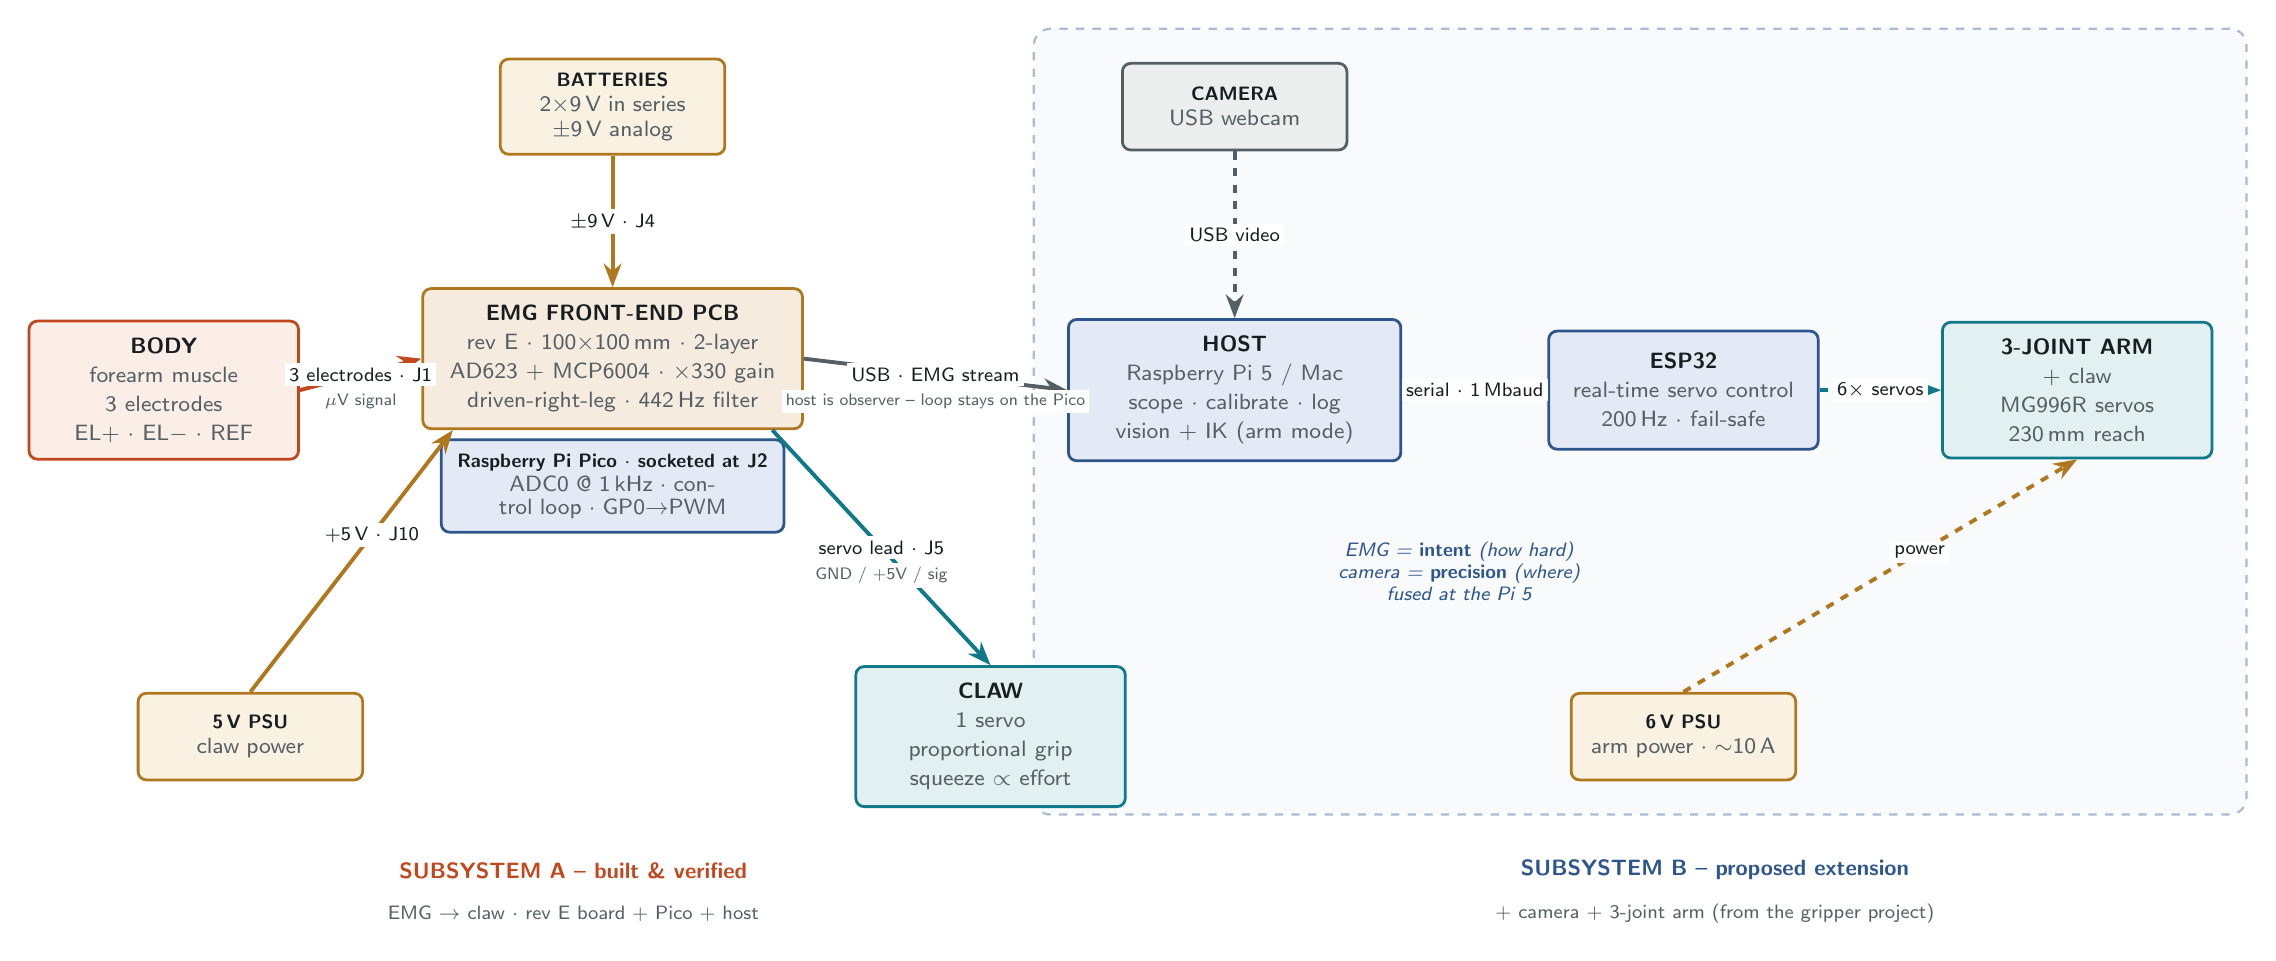
\begin{tikzpicture}[node distance=0pt]

% ================= NODES =================
% --- the EMG front-end board: the hub ---
\node[blk=emg, text width=4.4cm, fill=copperbg, draw=amber] (pcb) at (6,9.4)
  {EMG FRONT-END PCB\dl{rev E $\cdot$ 100$\times$100\,mm $\cdot$ 2-layer}\dl{AD623 + MCP6004 $\cdot$ $\times$330 gain}\dl{driven-right-leg $\cdot$ 442\,Hz filter}};
% Pico daughter-board, socketed onto the PCB at J2
\node[small=comp, text width=4.0cm, fill=compbg, minimum height=0.9cm,
      below=3pt of pcb] (pico)
  {Raspberry Pi Pico $\cdot$ socketed at J2\dl{ADC0 @ 1\,kHz $\cdot$ control loop $\cdot$ GP0$\to$PWM}};

\node[blk=emg, fill=emgbg] (body) at (0.3,9)
  {BODY\dl{forearm muscle}\dl{3 electrodes}\dl{EL+ $\cdot$ EL$-$ $\cdot$ REF}};

\node[small=amber, fill=amberbg] (batt) at (6,12.6)
  {BATTERIES\dl{2$\times$9\,V in series}\dl{$\pm$9\,V analog}};

\node[small=amber, fill=amberbg] (psu5) at (1.4,4.6)
  {5\,V PSU\dl{claw power}};

\node[blk=teal, fill=tealbg] (claw) at (10.8,4.6)
  {CLAW\dl{1 servo}\dl{proportional grip}\dl{squeeze $\propto$ effort}};

\node[blk=comp, text width=3.8cm, fill=compbg] (host) at (13.9,9)
  {HOST\dl{Raspberry Pi 5 / Mac}\dl{scope $\cdot$ calibrate $\cdot$ log}\dl{vision + IK (arm mode)}};

\node[small=data, fill=databg] (cam) at (13.9,12.6)
  {CAMERA\dl{USB webcam}};

\node[blk=comp, fill=compbg] (esp) at (19.6,9)
  {ESP32\dl{real-time servo control}\dl{200\,Hz $\cdot$ fail-safe}};

\node[blk=teal, fill=tealbg] (arm) at (24.6,9)
  {3-JOINT ARM\dl{+ claw}\dl{MG996R servos}\dl{230\,mm reach}};

\node[small=amber, fill=amberbg] (bigpsu) at (19.6,4.6)
  {6\,V PSU\dl{arm power $\cdot$ $\sim$10\,A}};

% ================= EDGES =================
% -- built / designed: solid --
\draw[sig, emg]  (body.east) -- (pcb.west)
      node[lbl]{3 electrodes $\cdot$ J1}
      node[lbls, below=5pt]{$\mu$V signal};
\draw[sig, amber] (batt.south) -- (pcb.north)
      node[lbl]{$\pm$9\,V $\cdot$ J4};
\draw[sig, amber] (psu5.north) -- ($(pcb.south west)+(0.4,0)$)
      node[lbl,pos=0.6]{+5\,V $\cdot$ J10};
\draw[sig, teal]  ($(pcb.south east)+(-0.4,0)$) -- (claw.north)
      node[lbl,pos=0.5]{servo lead $\cdot$ J5}
      node[lbls,pos=0.5,below=5pt]{GND / +5V / sig};
\draw[sig, data]  (pcb.east) -- (host.west)
      node[lbl]{USB $\cdot$ EMG stream}
      node[lbls, below=5pt]{host is observer -- loop stays on the Pico};

% -- proposed integration: dashed --
\draw[sig, data, dashed] (cam.south) -- (host.north)
      node[lbl]{USB video};
\draw[sig, data, dashed] (host.east) -- (esp.west)
      node[lbl]{serial $\cdot$ 1\,Mbaud};
\draw[sig, teal, dashed] (esp.east) -- (arm.west)
      node[lbl]{6$\times$ servos};
\draw[sig, amber, dashed] (bigpsu.north) -- (arm.south)
      node[lbl,pos=0.6]{power};

% intent + precision annotation
\node[det, text width=3.6cm, align=center, text=comp] at (16.75,6.7)
  {\itshape EMG = \textbf{intent} (how hard)\\ camera = \textbf{precision} (where)\\ fused at the Pi 5};

% subsystem captions
\node[font=\footnotesize\bfseries, text=emg] at (5.5,2.9) {SUBSYSTEM A -- built \& verified};
\node[det] at (5.5,2.35) {EMG $\to$ claw $\cdot$ rev E board + Pico + host};
\node[font=\footnotesize\bfseries, text=comp] at (20,2.9) {SUBSYSTEM B -- proposed extension};
\node[det] at (20,2.35) {+ camera + 3-joint arm (from the gripper project)};

% dashed region behind subsystem B
\begin{scope}[on background layer]
  \node[rounded corners=6pt, draw=comp!40, line width=0.8pt, dash pattern=on 3pt off 3pt,
        fit=(cam)(esp)(arm)(bigpsu)(host), inner sep=12pt, fill=comp!3] {};
\end{scope}

\end{tikzpicture}%
}

\vspace{4pt}

% ---- legend + status --------------------------------------------------
\resizebox{\textwidth}{!}{%
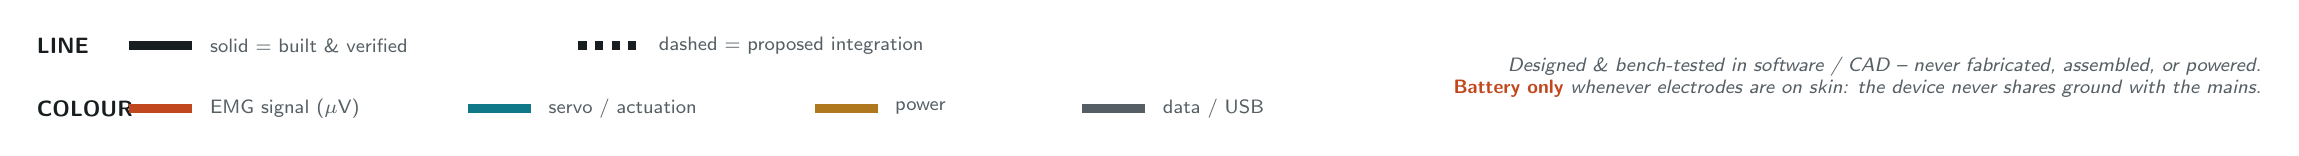
\begin{tikzpicture}
  \tikzset{sw/.style={line width=3pt}}
  % line-style key
  \node[font=\footnotesize\bfseries, text=ink, anchor=west] at (0,0.4) {LINE};
  \draw[sw, ink] (1.3,0.4)--(2.1,0.4); \node[anchor=west,font=\scriptsize,text=soft] at (2.2,0.4){solid = built \& verified};
  \draw[sw, ink, dashed] (7.0,0.4)--(7.8,0.4); \node[anchor=west,font=\scriptsize,text=soft] at (7.9,0.4){dashed = proposed integration};
  % colour key
  \node[font=\footnotesize\bfseries, text=ink, anchor=west] at (0,-0.4) {COLOUR};
  \draw[sw, emg]  (1.3,-0.4)--(2.1,-0.4); \node[anchor=west,font=\scriptsize,text=soft] at (2.2,-0.4){EMG signal ($\mu$V)};
  \draw[sw, teal] (5.6,-0.4)--(6.4,-0.4); \node[anchor=west,font=\scriptsize,text=soft] at (6.5,-0.4){servo / actuation};
  \draw[sw, amber](10.0,-0.4)--(10.8,-0.4);\node[anchor=west,font=\scriptsize,text=soft] at (10.9,-0.4){power};
  \draw[sw, data] (13.4,-0.4)--(14.2,-0.4);\node[anchor=west,font=\scriptsize,text=soft] at (14.3,-0.4){data / USB};
  % status, right-aligned
  \node[anchor=east, font=\scriptsize\itshape, text=soft, align=right] at (28.5,0)
    {Designed \& bench-tested in software / CAD -- never fabricated, assembled, or powered.\\
     \textbf{\color{emg}Battery only} whenever electrodes are on skin: the device never shares ground with the mains.};
\end{tikzpicture}%
}

\end{center}
\end{document}
